\section{Editor}
\label{sec:editor}
%TODO: May need newpage for layout reasons! Figures are booped up atm.
The editor, which allows the users to program their cells, is implemented with the following user interface, shown in \autoref{fig:editor_layout}

\begin{figure}[ht]
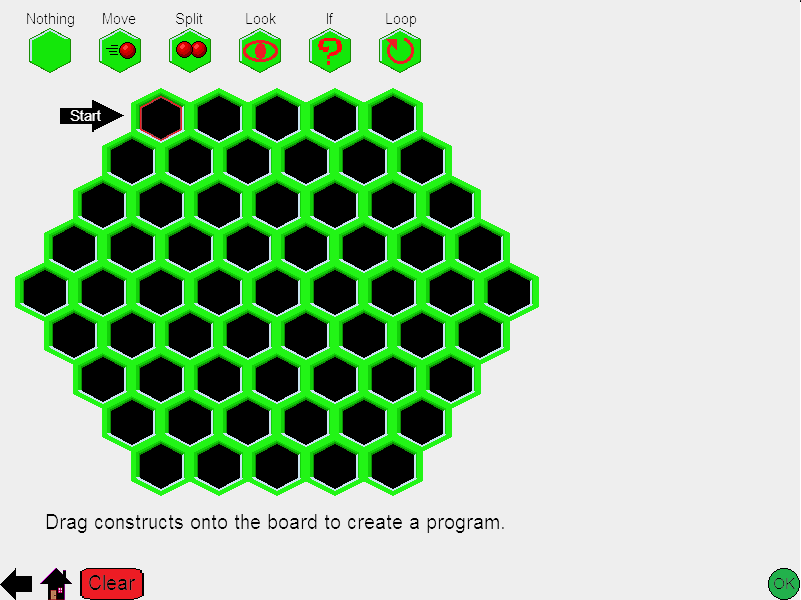
\includegraphics[width=\textwidth]{img/editor_layout.png}
\caption{Editor layout without form}
\label{fig:editor_layout}
\end{figure}

The editor constructs are draggable and will snap into tiles on the board once they are dropped there. Dragging a constructs creates a copy of the graphics to give the user a feeling of literally building a program. Once the user drops the construct on the board an HTML form will pop up, allowing the user to customize the construct. Below, in \autoref{fig:form_layout} is shown the form for the loop construct:

\begin{figure}[ht]
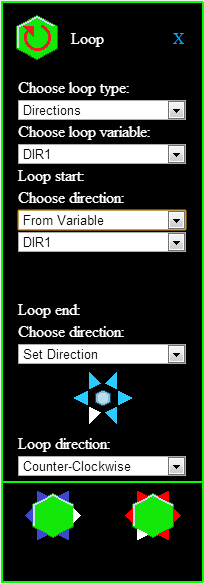
\includegraphics[scale=1]{img/editor_loop_form.png}
\caption{Form layout for the loop construct}
\label{fig:form_layout}
\end{figure}

When a tile is dragged the Drag class saves the type of instruction while the user is dragging it. Once it is dropped on the grid the Drag class sends the coordinates of the drop and the instruction type to the Editor class, which then adds it in the Program class. 

When the instruction is customized in the form it is immediately updated in the Program class. This means that the user can input e.g. a number and, without pressing save or enter, simply close the form and the input will be there the next time the form is brought up, which is done via clicking the tile on the grid.

The instructions are transferred as JS objects with a rather similar structure; below is an example of an instruction, specifically the "loop":

\begin{lstlisting}[language=javascript]
Instruction.loop = function()
{
	return {
		'type': 'loop',

		'expr_type': 'DIR',
		'variable': 'DIR1',
		'start':
		{
			'source': 'explicit',
			'value': 'R'
		},
		'end':
		{
			'source': 'explicit',
			'value': 'DL'
		},
		'increment': 'DV_COUNTERCLOCKWISE',
		
		'continue': 'R',
		'divert': 'DL'
	};
};
\end{lstlisting}

All instructions have a type, in this case loop, and a direction to continue in. Some instructions (if and loop) have two directions to continue in due to their behaviour. In between the type and the continue directions is the customizable information for that type. The only type of instruction that does not have any customization in between type and continue is nop.